\section{Problem 1}

\subsection{Part A}
Listing \ref{problem1:code} shows my Ruby implementation of the Needleman-Wunsch
algorithm. 

\lstinputlisting[language=Ruby, caption=Ruby implementation of
Needleman-Wunsch sequence alignment,
label=problem1:code]{6.878/ps1/code/ps1-seqalign.rb}

The implementation loosely follows the provided Python implementation, with the
major difference that it reads the scoring matrix from a file. Listing
\ref{problem1:a_scores} shows the scoring file translated from the provided
Python implementation.

\lstinputlisting[float=hbp, language=C, caption=The scoring matrix translated
from the Python code, label=problem1:a_scores]{6.878/ps1/code/a_scores.txt}

Figure \ref{problem1:solution} shows an optimal alignment of AGGTGAT with
AGTAA. Figures \ref{problem1:scores} and \ref{problem1:parents} show the
alignment scores and the information needed to reconstruct the optimal
alignment.

\begin{figure}[hbp]
\center \begin{verbatim}
A-GTGA-
AGGTAAT
\end{verbatim}

\caption{An optimal alignment of AGGTGAT with AGTAA}
\label{problem1:solution}
\end{figure}

\begin{figure}[hbp]
\center \begin{tabular}{|r|r|r|r|r|r|r|}
\hline
 & | & A & G & T & A & A\\
\hline
| & 0 & -4.0 & -8.0 & -12.0 & -16.0 & -20.0\\
\hline
A & -4.0 & 3 & -1.0 & -5.0 & -9.0 & -13.0\\
\hline
G & -8.0 & -1.0 & 6 & 2.0 & -2.0 & -6.0\\
\hline
G & -12.0 & -5.0 & 2.0 & 4 & 1.0 & -3.0\\
\hline
T & -16.0 & -9.0 & -2.0 & 5.0 & 2 & -1.0\\
\hline
G & -20.0 & -13.0 & -6.0 & 1.0 & 4.0 & 1\\
\hline
A & -24.0 & -17.0 & -10.0 & -3.0 & 4.0 & 7.0\\
\hline
T & -28.0 & -21.0 & -14.0 & -7.0 & 0.0 & 3.0\\
\hline
\end{tabular}

\caption{Alignment scores for AGGTGAT vs AGTAA}
\label{problem1:scores}
\end{figure}

\begin{figure}[hbp]
\center \begin{tabular}{|r|r|r|r|r|r|r|}
\hline
 & | & A & G & T & A & A\\
\hline
| & $\cdot$ & $\leftarrow$ & $\leftarrow$ & $\leftarrow$ & $\leftarrow$ & $\leftarrow$\\
\hline
A & $\uparrow$ & $\nwarrow$ & $\leftarrow$ & $\leftarrow$ & $\nwarrow$ & $\nwarrow$\\
\hline
G & $\uparrow$ & $\uparrow$ & $\nwarrow$ & $\leftarrow$ & $\leftarrow$ & $\leftarrow$\\
\hline
G & $\uparrow$ & $\uparrow$ & $\nwarrow$ & $\nwarrow$ & $\nwarrow$ & $\nwarrow$\\
\hline
T & $\uparrow$ & $\uparrow$ & $\uparrow$ & $\nwarrow$ & $\nwarrow$ & $\nwarrow$\\
\hline
G & $\uparrow$ & $\uparrow$ & $\nwarrow$ & $\uparrow$ & $\nwarrow$ & $\nwarrow$\\
\hline
A & $\uparrow$ & $\nwarrow$ & $\uparrow$ & $\uparrow$ & $\nwarrow$ & $\nwarrow$\\
\hline
T & $\uparrow$ & $\uparrow$ & $\uparrow$ & $\nwarrow$ & $\uparrow$ & $\uparrow$\\
\hline
\end{tabular}

\caption{Solution reconstruction data  for AGGTGAT vs AGTAA}
\label{problem1:parents}
\end{figure}

\subsection{Part B}
The Ruby implementation does not need to be modified. It is sufficient to
change the scoring matrix to reflect the Hamilton distance between genes.
Listing \ref{problem1:b_scores} shows the changed score file. The resulting
score's absolute magnitude reflects the number of base mutations (insertions,
deletions, substitutions) between the two genes. 

\lstinputlisting[float=hbp, language=C, caption=The scoring matrix used to
compute the distance between two genes,
label=problem1:b_scores]{6.878/ps1/code/b_scores.txt}

\subsection{Part C}
Running the program as described above yields a score of -111.

\subsection{Part D}
Aligning the human versions of HoxA13 and HoxD13 yields a score of -467.
Aligning the mouse version of the same genes yields a score of -471. I use the
mean score.

Aligning the human version of HoxD13 with the mouse version of HoxD13 yields a
score of -154. The big difference between this and the score obtained in part B
is slightly disheartening, and I'll definitely use the mean score. The
difference probably suggests that the scoring matrix is not very good.

Assuming that that mammalian genomes undergo a constant rate of mutations over
time, we find that the HoxA13 and HoxD13 genes have probably diverged

$$
\frac{467 + 471}{2} \cdot \frac{2}{111 + 154} \cdot {70 \textrm{ million years}}
\approx 248 \textrm{ million years}
$$

Note that, for simplification, the scoring matrix in listing
\ref{problem1:b_scores} assumes that all base mutations (insertions, deletions,
substitutions) are equally probable. This is known not to be the case.


\section{Problem 2}

The recurrence is as follows:

$$
F(i, j, k) = \max \left\{
\begin{array}{l}
F(i - 1, j, k) + s(i, \cdot, \cdot) \\
F(i, j - 1, k) + s(\cdot, j, \cdot) \\
F(i, j, k - 1) + s(\cdot, \cdot, k) \\
F(i - 1, j - 1, k) + s(i, j, \cdot) \\
F(i, j - 1, k - 1) + s(\cdot, j, k) \\
F(i - 1, j, k - 1) + s(i, \cdot, k) \\
F(i - 1, j - 1, k - 1) + s(i, j, k)
\end{array}
\right.
$$

The initial conditions are $F(0, 0, 0) = 0$, $F(i, j, k) = -\infty$ if $i <
0$ or $j < 0$ or $k < 0$, and $s(i, j, k) = -\infty$ if $i \cdot j \cdot k = 0$.

\section{Problem 3}

\subsection{Part A}

The program's output is reproduced in figure \ref{problem3:exact30}.

\begin{figure}[htb]
  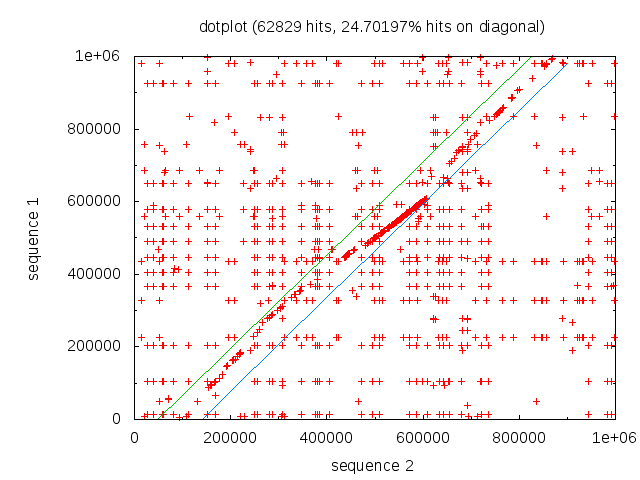
\includegraphics[width=6.8in]{6.878/ps1/figs/p3_exact30.png}
  \caption{Dotplot for all exact matching 30-mers.}
  \label{problem3:exact30}.
\end{figure}

\subsection{Part B}

The key observation for my solution is that all the required modifications are
still exact matching problems, but the subsequence of bases that have to match
isn't continuous. So, it is sufficient to modify the code to hash the
subsequences that have to match. Listing \ref{problem3:code} shows the
code changes needed to produce plots modifications i, ii, iii, and iv.

\begin{lstlisting}[language=Python, caption=The scoring matrix used to
compute the distance between two genes, label=problem3:code]
    # length of hash key
    kmerlen = 30
    # stride of hash key  # ADDED
    kmerstep = 1          # ADDED
    
    # hash table for finding hits
    lookup = {}
    
    # store sequence hashes in hash table
    print "hashing seq1..."
    for i in xrange(len(seq1) - kmerlen + 1):
        key = seq1[i:i+kmerlen:kmerstep]        # CHANGED
        lookup.setdefault(key, []).append(i)    # CHANGED



    # look up hashes in hash table
    print "hashing seq2..."
    hits = []
    for i in xrange(len(seq2) - kmerlen + 1):
        key = seq2[i:i+kmerlen:kmerstep]        # CHANGED
        
        # store hits to hits list
        for hit in lookup.get(key, []):
            hits.append((i, hit))
\end{lstlisting}

The script above outputs the original plot. The following values for kmerlen
and kmerstep produce the plots for modifications i-iv:
\begin{enumerate}
  \item [i.] kmerlen = 100, kmerstep = 1
  \item [ii.] kmerlen = 60, kmerstep = 2
  \item [iii.] kmerlen = 90, kmerstep = 3
  \item [iv.] kmerlen = 120, kmerstep = 4 
\end{enumerate}

\subsection {Part C}

\subsection {Part D}

\begin{tabular}{|l|r|r|}
\hline
Original & 62829 & 24.70\% \\
\hline
Modification i & & \\
\hline
Modification ii & & \\
\hline
Modification iii & & \\
\hline
Modification iv & & \\
\hline
Modification v & & \\
\hline
\end{tabular}
\end{tabular}

\subsection {Part E}
